\documentclass[11pt,a4paper]{article}

\usepackage[utf8]{inputenc}
\usepackage{parskip}
\usepackage{tabularx}
\usepackage{amsmath}
\usepackage{amssymb}
\usepackage{amsthm}
\usepackage{geometry}
\usepackage{booktabs}
\usepackage{centernot}
\usepackage{hyperref}
\usepackage{eufrak}
\usepackage{graphicx}
\graphicspath{{pics/}}
\geometry{a4paper, left=20mm, right=20mm, top=20mm, bottom=20mm}

\usepackage{fancyhdr}
\pagestyle{fancy}
\lhead{Anthony Catterwell}
\chead{\textsc{University of Edinburgh}}
\rhead{Operating Systems}

\title{Operating Systems Lecture Notes}
\author{Anthony Catterwell}

\begin{document}
\maketitle
\tableofcontents

\break{}

\section{Introduction}

\section{Operating System Structure}

\subsection{Architectural impact}

\textbf{Architectural features affecting OS\emph{s}}
\begin{itemize}
    \item These features were built primarily to support OS\emph{s}:
        \begin{itemize}
            \item timer (clock) operationg
            \item synchronisation instructions
            \item memory protection
            \item I/O control operations
            \item interrupts and exceptions
            \item protected modes of operation (kernel vs.\ user mode)
            \item privileged instructions
            \item system calls (including software interrupts)
            \item virtualisation architectures
        \end{itemize}
    \item ASPLOS
\end{itemize}

\subsection{User operating interaction}

\subsubsection{User v.s.\ kernel}

\textbf{Privileged instructions}
\begin{itemize}
    \item Some instructions are restricted to the OS
        \begin{itemize}
            \item known as \emph{privileged} instructions
        \end{itemize}
    \item Only the OS can:
        \begin{itemize}
            \item directly access I/O devices
            \item manipulate memory state management (page table pointers, TLB loads, etc.)
            \item manipulate special \emph{mode bits} (interrupt priority level)
        \end{itemize}
    \item Restrictions provide safety and security
\end{itemize}

\textbf{OS protections}
\begin{itemize}
    \item So how does the process know if a privileged instruction should be executed?
        \begin{itemize}
            \item the architecture must support at least two modes of operation:
                kernel mode, and user mode
            \item mode is set by status bit in a protected processor register.
                \begin{itemize}
                    \item user programs execute in user mode
                    \item OS executes in kernel (privileged) mode (OS == kernel)
                \end{itemize}
            \item Privileged instructions can only be executed in kernel (privileged) mode
                \begin{itemize}
                    \item if code running in user mode attempts to execute a privileged
                        instruction, the illegal execution trap.
                \end{itemize}
        \end{itemize}
\end{itemize}

\textbf{Crossing protection boundaries}
\begin{itemize}
    \item So how do user programs do something privileged?
        \begin{itemize}
            \item e.g.\ how can you write to a disk if you can't execute any I/O instructions?
        \end{itemize}
    \item User programs must call on OS procedure --- that is to ask the OS to do it for them.
        \begin{itemize}
            \item OS defines a set of system calls
            \item User-mode program executes system call instruction
        \end{itemize}
    \item Syscall instruction
        \begin{itemize}
            \item like a protected procedure call
        \end{itemize}
\end{itemize}

\subsubsection{Syscall}

\textbf{Syscall}
\begin{itemize}
    \item The syscall instruction \emph{atomically}:
        \begin{itemize}
            \item saves the current PC
            \item sets the execution mode to privileged
            \item sets the PC to a handler address
        \end{itemize}
    \item Similar to a procedure call
        \begin{itemize}
            \item Caller puts arguments in a place the callee expects (registers, or stack)
                \begin{itemize}
                    \item One of the args is a syscall number, indicating which OS function
                        to invoke
                \end{itemize}
            \item Callee (OS) saves caller's state (registers, other control states) so it can
                use the CPU
            \item OS function code runs
                \begin{itemize}
                    \item OS must verify caller's arguments (e.g.\ pointers)
                \end{itemize}
            \item OS returns using a special instruction
                \begin{itemize}
                    \item Automatically sets PC to return address and sets execution mode to
                        user.
                \end{itemize}
        \end{itemize}
\end{itemize}

\begin{center}{}
    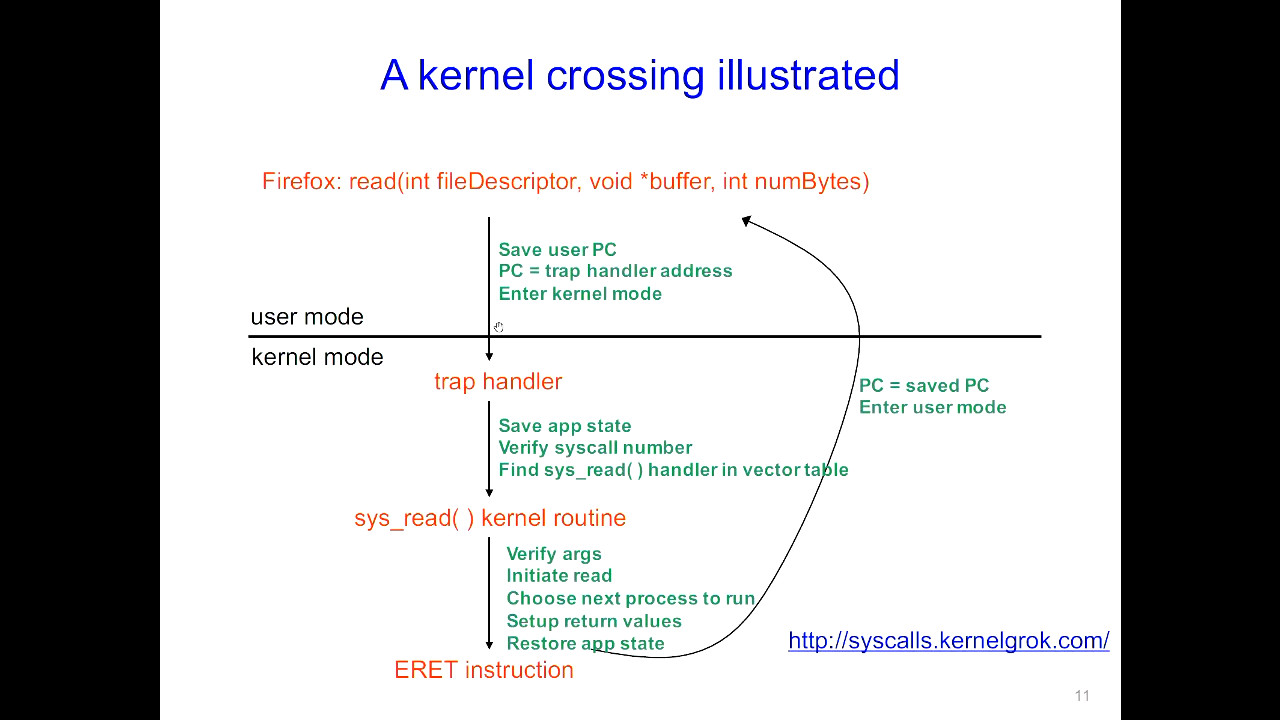
\includegraphics[height=270]{a-kernel-crossing-illustrated.jpg}
\end{center}

\textbf{System call issues}
\begin{itemize}
    \item A syscall is not a subroutine call, with the caller specifying the next PC.\
        \begin{itemize}
            \item the caller knows where the subroutines are located in memory;
                therefore they can be the target of an attack.
        \end{itemize}
    \item The kernel saves state?
        \begin{itemize}
            \item Prevents overwriting of values
        \end{itemize}
    \item The kernel verify arguments
        \begin{itemize}
            \item Prevents buggy code crashing the system
        \end{itemize}
    \item Referring to kernel objects as arguments
        \begin{itemize}
            \item Data copied between user buffer and kernel buffer.
        \end{itemize}
\end{itemize}

\textbf{Exception handling and protection}
\begin{itemize}
    \item \emph{All} entries to the OS occur via the mechanism just shown
        \begin{itemize}
            \item Acquiring privileged mode and branching to the trap handler are inseparable
        \end{itemize}
    \item Terminology
        \begin{itemize}
            \item \emph{Interrupt}: asynchronous; caused by an external device
            \item \emph{Exception}: synchronous; unexpected problem with instruction
            \item \emph{Trap}: synchronous; intended transition to OS due to an instruction
        \end{itemize}
        In all three cases, they are instances of where something strange happens,
        and the OS takes control: whether by accident, or by intention.
    \item Privileged instructions and resources are the basis for most everything:
        memory protection, protected I/O, limiting user resource consumption.
\end{itemize}

\subsection{Operating System structure}

\subsubsection{Layers}

\textbf{Operating System structure}
\begin{itemize}
    \item The OS sits between application programs and the hardware
        \begin{itemize}
            \item it mediates access and abstracts away ugliness
            \item programs request services via traps or exceptions
            \item devices request attention via interrupts
        \end{itemize}
\end{itemize}

\textbf{Operating system design and implementation}
\begin{itemize}
    \item Design and implementation of OS not ``solvable'', but some approaches have proven
        successful.
    \item Internal structure of different OS\emph{s} can vary widely.
    \item Start the design by defining goals and specifications.
    \item Affected by choice of hardware, type of system.
    \item \emph{User} goals, and \emph{system} goals
        \begin{itemize}
            \item User goals: OS should be convenient to use, easy to learn, reliable, safe,
                and fast
            \item System goals: OS should be easy to design, implement, and maintain,
                as well as flexible, reliable, error-free, and efficient.
        \end{itemize}
    \item Important principle to separate
        \begin{itemize}
            \item \textbf{Policy}: \emph{What} will be done?
            \item \textbf{Mechanism}: \emph{How} to do it?
        \end{itemize}
    \item Mechanisms determine how to do something, policies decide what will be done.
    \item The separation of policy from mechanism is a very important principle,
        it allows maximum flexibility if policy decisions are to be changed later
        (e.g.\ timer).
    \item Specifying and designing an OS is a highly creative task of
        \emph{software engineering}.
\end{itemize}

\textbf{System layers}
\begin{center}{}
    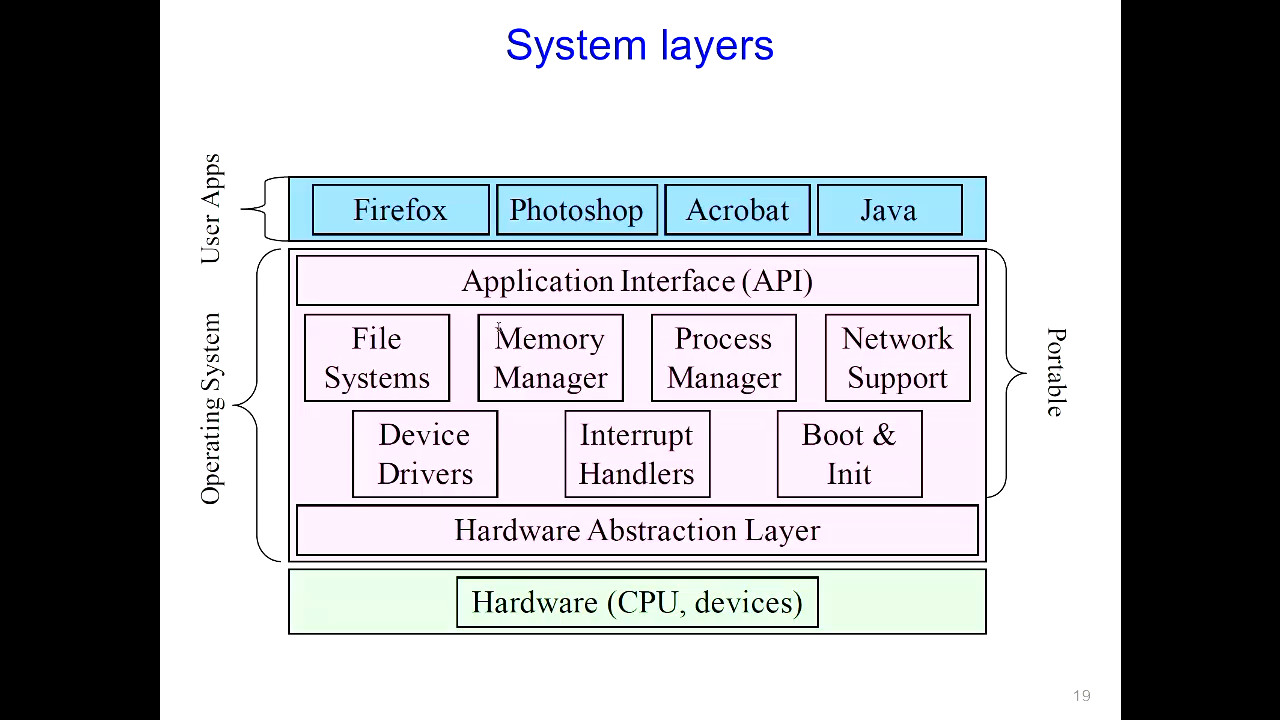
\includegraphics[height=280]{system-layers.jpg}
\end{center}

\textbf{Major OS components}
\begin{itemize}
    \item processes
    \item memory
    \item I/O
    \item secondary storage
    \item file systems
    \item protection
    \item shells
    \item GUI
    \item networking
\end{itemize}

\textbf{OS structure}

\begin{itemize}
    \item There's no clear hierarchy within an OS --- each of them needs access to different
        things.
    \item An OS consists of all these components, plus:
        \begin{itemize}
            \item many other components
            \item system programs (privileged, and non-privileged)
        \end{itemize}
    \item Major issue:
        \begin{itemize}
            \item how do we organize all this?
            \item what are all of the code modules, and where do they exist?
            \item how do they cooperate?
        \end{itemize}
    \item Massive software engineering and design problem
        \begin{itemize}
            \item design a large, complex program that:
                performs well, is reliable, is extensible, and is backwards compatible.
        \end{itemize}
\end{itemize}

\subsubsection{Examples}

\textbf{Monolithic design}
\begin{itemize}
    \item Traditionally, OS\emph{s} (like UNIX) were built as a \emph{monolithic} entity
        User programs | OS (everything) | hardware
    \item Major advantage: cost of module interactions is low (procedure call)
    \item Disadvantages:
        \begin{itemize}
            \item hard to understand
            \item hard to modify
            \item unreliable (no isolation between system modules)
            \item hard to maintain
        \end{itemize}
    \item What is the alternative? \\
        Find a way to organise the OS in order to simplify its design and implementation.
\end{itemize}

\textbf{Layering}
\begin{itemize}
    \item The traditional approach is layering
        \begin{itemize}
            \item implement OS as a set of layers
            \item each layer presents an enhanced \emph{virtual machine} to the layer above
        \end{itemize}
    \item The first description of this approach was Dijkstra's THE system
        \begin{itemize}
            \item Layer 5: \emph{Job managers} execute users' programs
            \item Layer 4: \emph{Device managers} handle devices and provide buffering
            \item Layer 3: \emph{Console manager} implements virtual consoles
            \item Layer 2: \emph{Page manager} implements virtual memories for each process
            \item Layer 1: \emph{Kernel} implements a virtual processor for each process
            \item Layer 0: \emph{Hardware}
        \end{itemize}
    \item Each layer can be tested and verified independently
    \item Imposes a hierarchical stricture
        \begin{itemize}
            \item but real systems are more complex:
                file systems require VM services (buffer);
                VM would like to use files for its backing store
            \item strict layering isn't flexible enough
        \end{itemize}
    \item Poor performance:
        each layer crossing has \emph{overhead} associated with it
    \item Disjunction between model and reality:
        systems modelled as layers, but not really built that way.
\end{itemize}

\textbf{Hardware abstraction layer}
\begin{itemize}
    \item An example of layering in modern operating systems
    \item Goal: separates hardware-specific routines from the \emph{core} OS
        \begin{itemize}
            \item Provides portability
            \item Improves readability
        \end{itemize}
\end{itemize}

\textbf{Microkernels}
\begin{itemize}
    \item Popular in the late 80s, early 90s
    \item Goal:
        minimize what happens in kernel;
        item organize rest of OS as user-level processes.
\item This results in:
    \begin{itemize}
        \item better reliability (isolation between components)
        \item easy of extension and customisation
        \item poor performance (user/kernel boundary crossings)
    \end{itemize}
\item First microkernel system was Hydra (CMU, 1970)
    \begin{itemize}
        \item Contemporaries: Mach (CMU), Chorus (French UNIX-like OS), OS X (Apple),
            in some ways NT (Microsoft)
    \end{itemize}
\end{itemize}

\begin{center}{}
    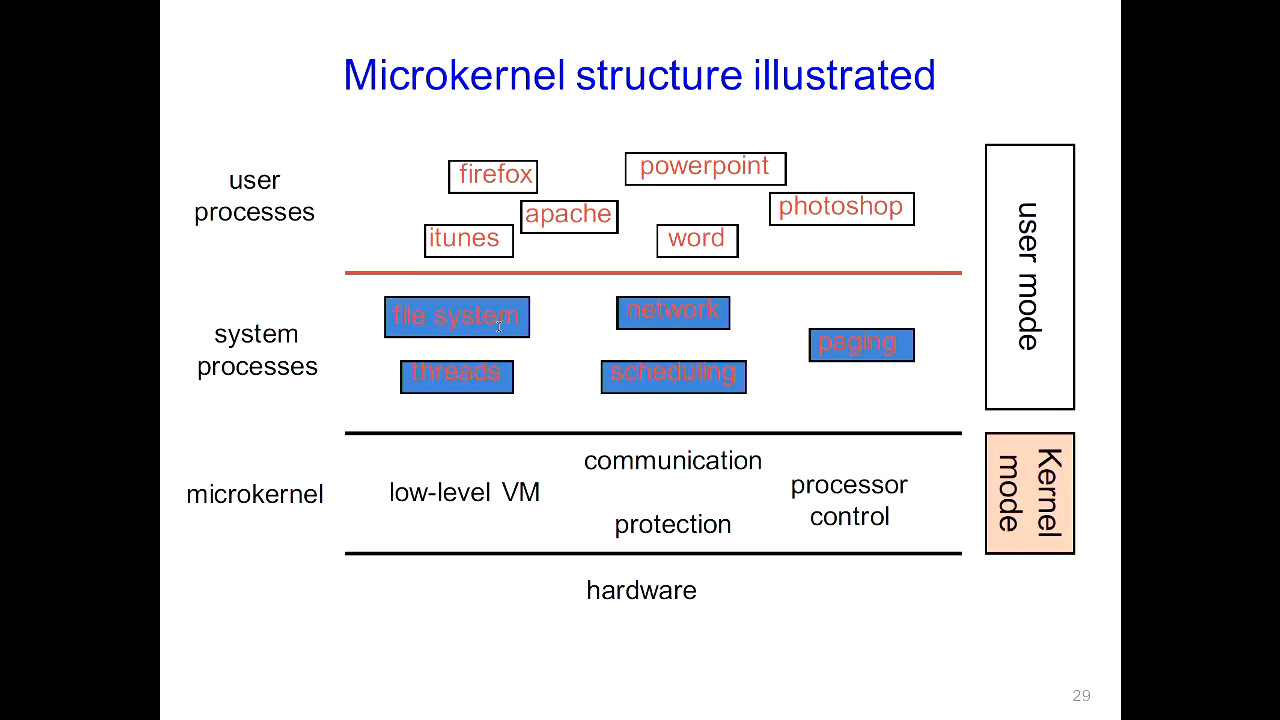
\includegraphics[height=270]{microkernel-structure-illustrated.jpg}
\end{center}

\textbf{Comparison of OS structures}

Windows

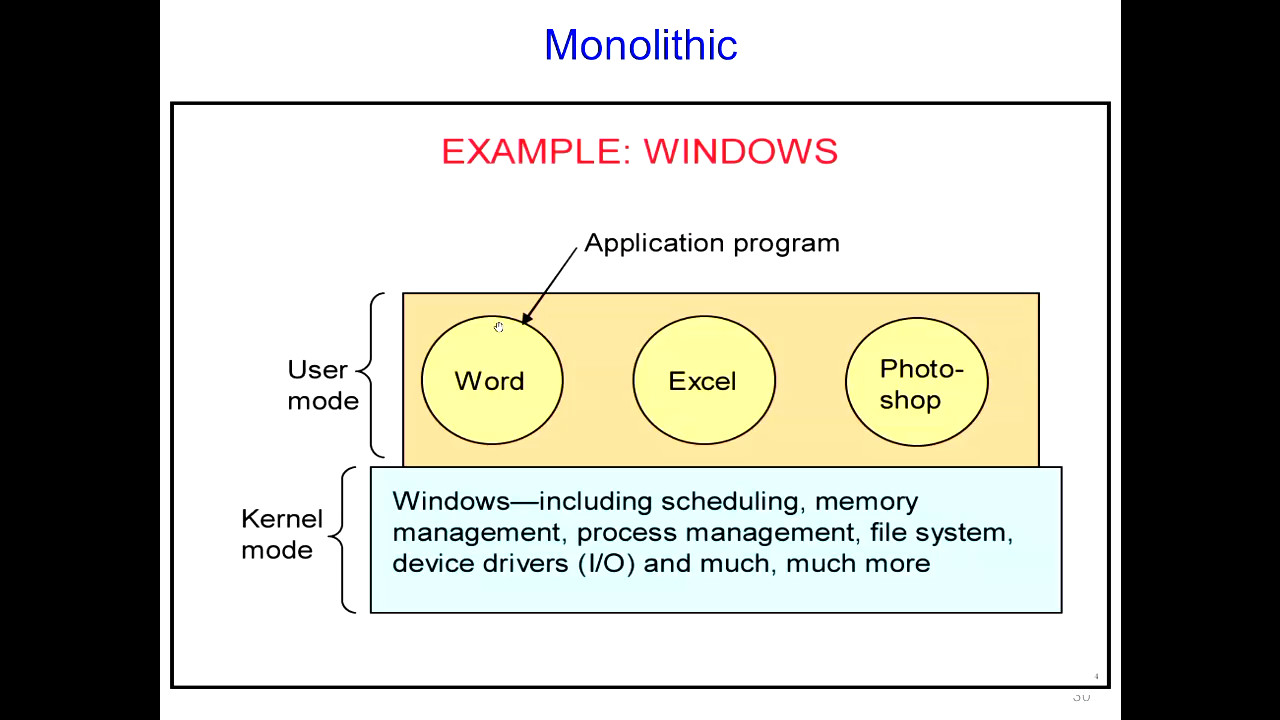
\includegraphics[height=270]{windows.jpg}

MINIX 3

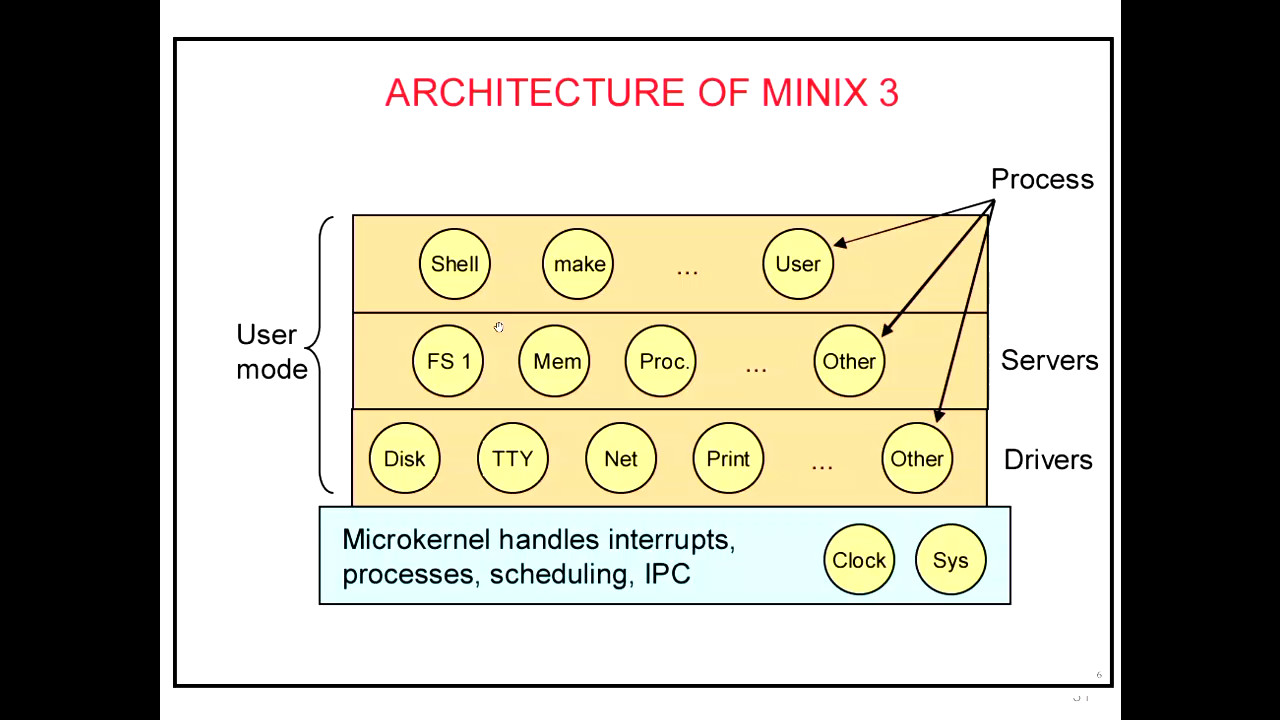
\includegraphics[height=270]{minix-3.jpg}

\textbf{Loadable kernel modules}

\begin{itemize}
    \item (Perhaps) the best practice for OS design
    \item Core services in the kernel, and others dynamically loaded
    \item Common implementations include: Solaris, Linux, etc.
    \item Advantages
        \begin{itemize}
            \item convenient: no need for rebooting for newly added modules
            \item efficient: no need for message passing unlike micro-kernel
            \item flexible: any module can call any other module unlike layered model
        \end{itemize}
\end{itemize}

\subsection{Summary}

\begin{itemize}
    \item Fundamental distinction between user and privileged mode supported by most hardware
    \item OS design has been an evolutionary process of trial and error.
    \item Successful OS designs have run the spectrum  from monolithic, to layered,
        to micro-kernels
    \item The role and design of an OS are still evolving
    \item It is impossible to pick one ``correct'' way to structure an OS
\end{itemize}

\break{}

\section{Processes}

\subsection{Process}

\textbf{What is a ``process''?}
\begin{itemize}
    \item The process is the OS\emph{s} abstraction for execution
        \begin{itemize}
            \item A process is a program in execution
        \end{itemize}
    \item Simplest (classic) case: a \emph{sequential process}
        \begin{itemize}
            \item An address space (an abstraction of memory)
            \item A single thread of execution (an abstraction of the CPU)
        \end{itemize}
    \item A sequential process is:
        \begin{itemize}
            \item The unit of execution
            \item The unit of scheduling
            \item The dynamic (active) execution context
                (as opposed to the program --- static, just a bunch of bytes)
        \end{itemize}

\end{itemize}

\textbf{What's ``in'' a process?}
\begin{itemize}
    \item A process consists of (at least):
        \begin{itemize}
            \item An \emph{address space}, containing:
                \begin{itemize}
                    \item the code (instructions) for the running program
                    \item the data for the running program (static data, heap data, stack)
                \end{itemize}
            \item \emph{CPU state}, consisting of:
                \begin{itemize}
                    \item the program counter (PC), indicating the next instruction;
                    \item the stack pointer;
                    \item other general purpose register values.
                \end{itemize}
            \item A set of \emph{OS resources}
                \begin{itemize}
                    \item open files, network connections, sound channels, \dots
                \end{itemize}
            \item In other words, everything needed to run the program
                (or to restart, if interrupted).
        \end{itemize}
\end{itemize}

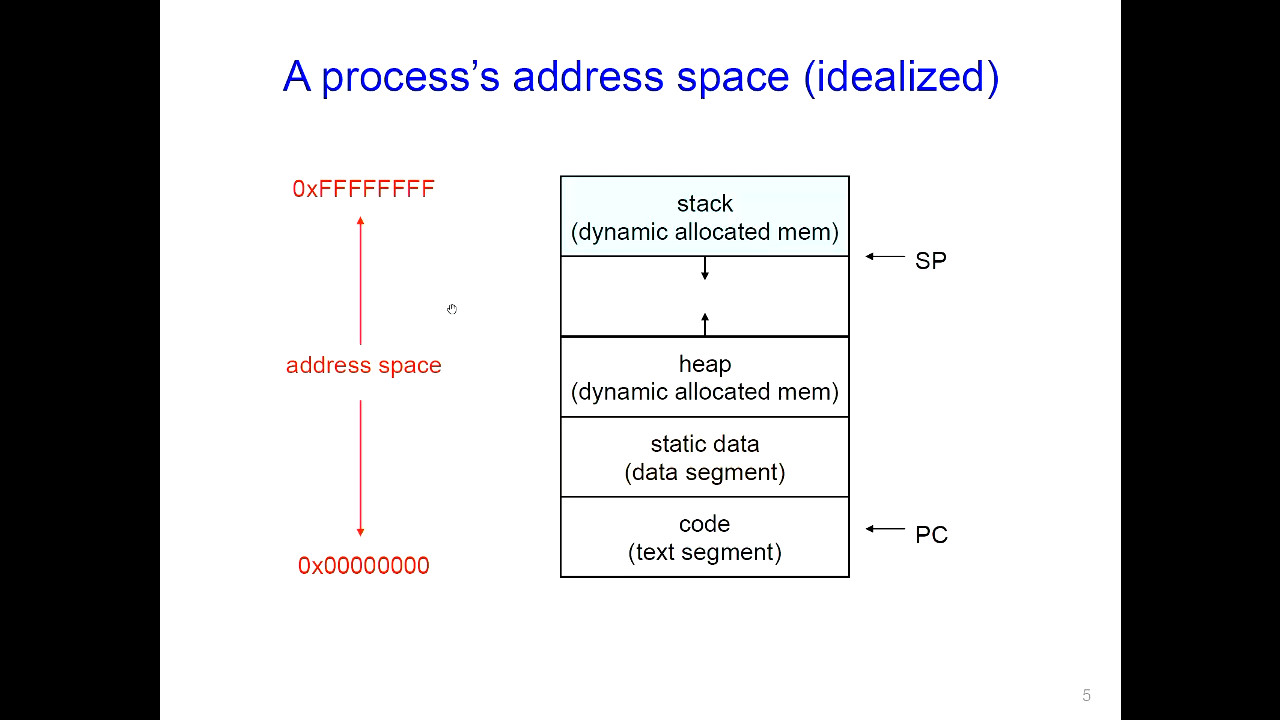
\includegraphics[height=280]{a-process-address-space.jpg}

\textbf{The OS process namespace}
\begin{itemize}
    \item The particulars depend on the specific OS, but the principles are general;
    \item The name for a process is called a \emph{process ID} (PID) (an integer);
    \item The PID namespace is global to the system;
    \item Operations that create processes return a PID (e.g.\ fork);
    \item Operations on processes take PIDs as an argument (e.g.\ kill, wait, nice).\
\end{itemize}

\subsection{Process control block}

\textbf{Representation of processes by the OS}
\begin{itemize}
    \item The OS maintains a data structure to keep track of a process's state
        \begin{itemize}
            \item called the \emph{process control block} (PCB)
                or \emph{process descriptor};
            \item identified by the PID.\
        \end{itemize}
    \item OS keeps all of a process's execution state in (or linked from) the PCB
        when the process isn't running
        \begin{itemize}
            \item PC, SP, registers, etc.
            \item when a process is unscheduled, the state is transferred out of the
                hardware into the PCB
            \item (when a process is running, its state is spread between the PCB and the CPU).
        \end{itemize}
\end{itemize}

\textbf{The PCB}
\begin{itemize}
    \item The PCB is a data structure with many, many fields
    \begin{itemize}
        \item PID
        \item parent PID
        \item execution state
        \item PC, SP, registers
        \item address space info
        \item UNIX user id, group id
        \item scheduling priority
        \item accounting info
        \item pointers for state queues
    \end{itemize}
\item In Linux:
    \begin{itemize}
        \item defined in \texttt{task\_struct (include/linux/sched.h)}
        \item Over 95 fields!
    \end{itemize}
\end{itemize}

\subsection{Process state \& context switch}

\textbf{PCBs and CPU state}
\begin{itemize}
    \item When a process is running, its CPU state is inside the CPU
        \begin{itemize}
            \item PC, SP, registers
            \item CPU contains current values
        \end{itemize}
    \item When the OS gets control because of a
        \begin{itemize}
            \item \emph{Trap}: program executes a syscall
            \item \emph{Exception}: program does something unexpected (e.g.\ page fault)
            \item \emph{Interrupt}: A hardware device requests service
        \end{itemize}
        the OS saves the CPU state of the running process in that process's PCB.\

    \item When the OS returns the process to the running state
        \begin{itemize}
            \item it loads the hardware registers with values from that process's PCB
            \item e.g.\ general purpose registers, SP, instruction pointer
        \end{itemize}
    \item This act of switching the CPU from one process to another is called a
        \emph{context switch}
        \begin{itemize}
            \item systems may do 100s or 1000s of switches per second;
            \item takes a few microseconds on today's hardware;
            \item still expensive relative to thread-based context switches.\
        \end{itemize}
    \item Choosing which process to run next is called \emph{scheduling}.\
\end{itemize}

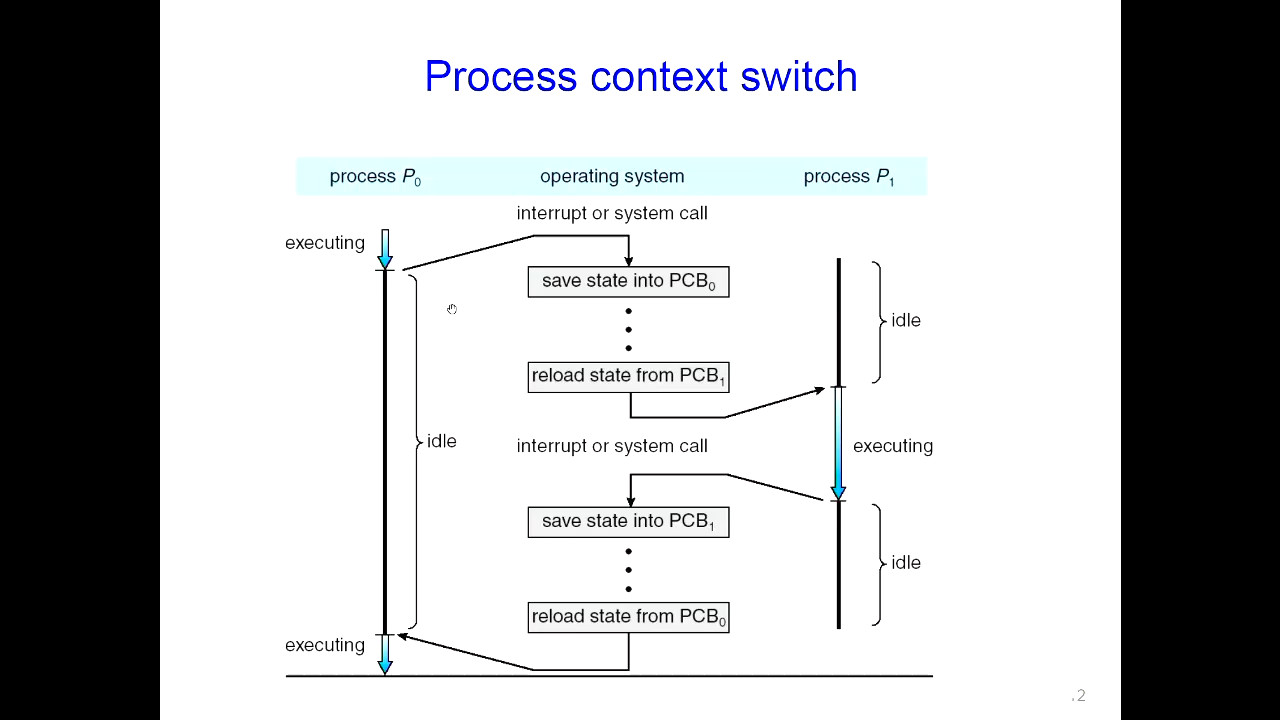
\includegraphics[height=280]{process-context-switch.jpg}

\textbf{Process execution states}
\begin{itemize}
    \item Each process has an \emph{execution state}, which indicates what it's currently doing
        \begin{itemize}
            \item \emph{ready}: waiting to be assigned to a CPU ---
                could run, but another process has the CPU;\
            \item \emph{running}: executing on a CPU ---
                it's the process that currently controls the CPU;\
            \item \emph{waiting} (aka ``blocked''): waiting for an event, e.g.\ I/O completion,
                or a messing from (or the completion of) another process ---
                cannot make progress until the event happens.
        \end{itemize}
    \item As a process executes, it moves from state to state
        \begin{itemize}
            \item UNIX:\ run \texttt{top}, STAT column shows current state
            \item which state is a process most of the time?
        \end{itemize}
\end{itemize}

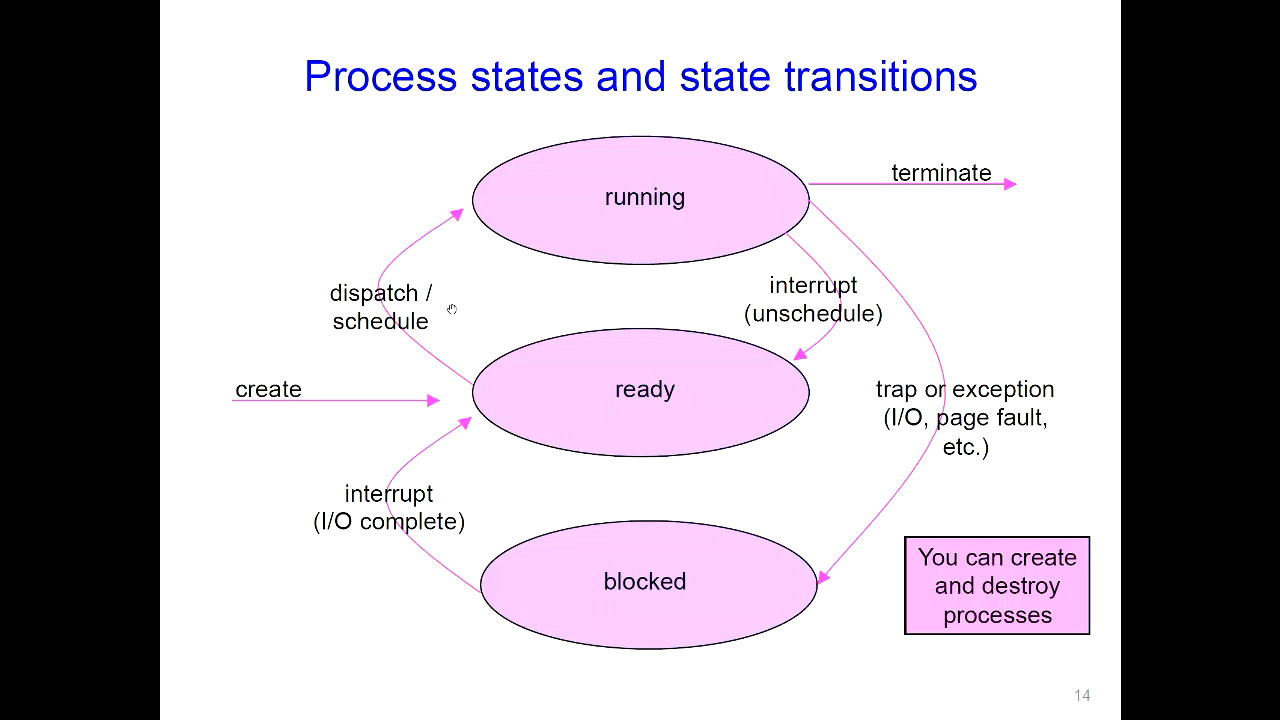
\includegraphics[height=280]{process-states-and-state-transitions.jpg}

\textbf{State queues}
\begin{itemize}
    \item The OS maintains a collection of queues that represent the state of all processes in
        the system
        \begin{itemize}
            \item typically one queue for each state (e.g.\ ready, waiting, \dots);
            \item each PCB is queued onto a state queue according to the current state of the
                process it represents;
            \item as a process changes state, its PCB is unlinked from one queue,
                and linked onto another.
        \end{itemize}
    \item The PCBs are moved between queues, which are represented as linked lists.
    \item There may be many wait queues, one for each type of wait
        (particular device, timer, message, \dots).
\end{itemize}

\textbf{PCBs and state queues}
\begin{itemize}
    \item PCBs are data structures
        \begin{itemize}
            \item dynamically allocated inside OS memory.
        \end{itemize}
    \item When a process is created:
        \begin{itemize}
            \item OS allocates a PCB for it;
            \item OS initializes PCB;\
            \item (OS does other things not related to the PCB);
            \item OS puts PCB on the correct queue.
        \end{itemize}
    \item As a process computes:
        \begin{itemize}
            \item OS moves its PCB from queue to queue.
        \end{itemize}
    \item When a process is terminated:
        \begin{itemize}
            \item PCB may be retained for a while (to receive signals, etc.)
            \item eventually, OS deallocates the PCB.\
        \end{itemize}
\end{itemize}

\subsection{Process creation and termination}

\textbf{Process creation}
\begin{itemize}
    \item New processes are created by existing processes
        \begin{itemize}
            \item creator is called the \emph{parent};
            \item created process is called the \emph{child};\\\
                UNIX:\ do \texttt{ps -ef}, look for PPID field
            \item what creates the first process, and when? \\
                on UNIX, this first process is init; \\
                on many Linux distributions, this is SystemD or Runit (on Void).
        \end{itemize}
\end{itemize}

\textbf{Process creation semantics}
\begin{itemize}
    \item (Depending on the OS) child processes inherit certain attributes of the parent.
        E.g.
        \begin{itemize}
            \item Open file table: implies \texttt{stdin}/\texttt{stdout}/\texttt{stderr};
            \item On some systems, resource allocation to parent may be divided among children.
        \end{itemize}
    \item (In Unix) when a child is created, the parent may either wait for the child to
        finish, or continue in parallel.
\end{itemize}

\textbf{UNIX process creation details}
\begin{itemize}
    \item UNIX process creation through \texttt{fork} system call
        \begin{itemize}
            \item creates and initializes a new PCB
                \begin{itemize}
                    \item initializes kernel resources of new process with resources of parent
                        (e.g.\ open files)
                    \item initializes PC, SP to be same as parent.
                \end{itemize}
            \item creates a new address space
                \begin{itemize}
                    \item initialises new address space with a copy of the entire contents of
                        the address space of the parent
                \end{itemize}
            \item places new PCB on the ready queue.
        \end{itemize}
    \item the \texttt{fork} system call ``returns twice''
        \begin{itemize}
            \item once into the parent, and once into the child
                \begin{itemize}
                    \item returns the child's PID to the parent
                    \item returns \texttt{0} to the child
                \end{itemize}
        \end{itemize}
    \item \texttt{fork} = ``clone me''. \\
        The return value is used to determine whether we're the clone or the original.
\end{itemize}

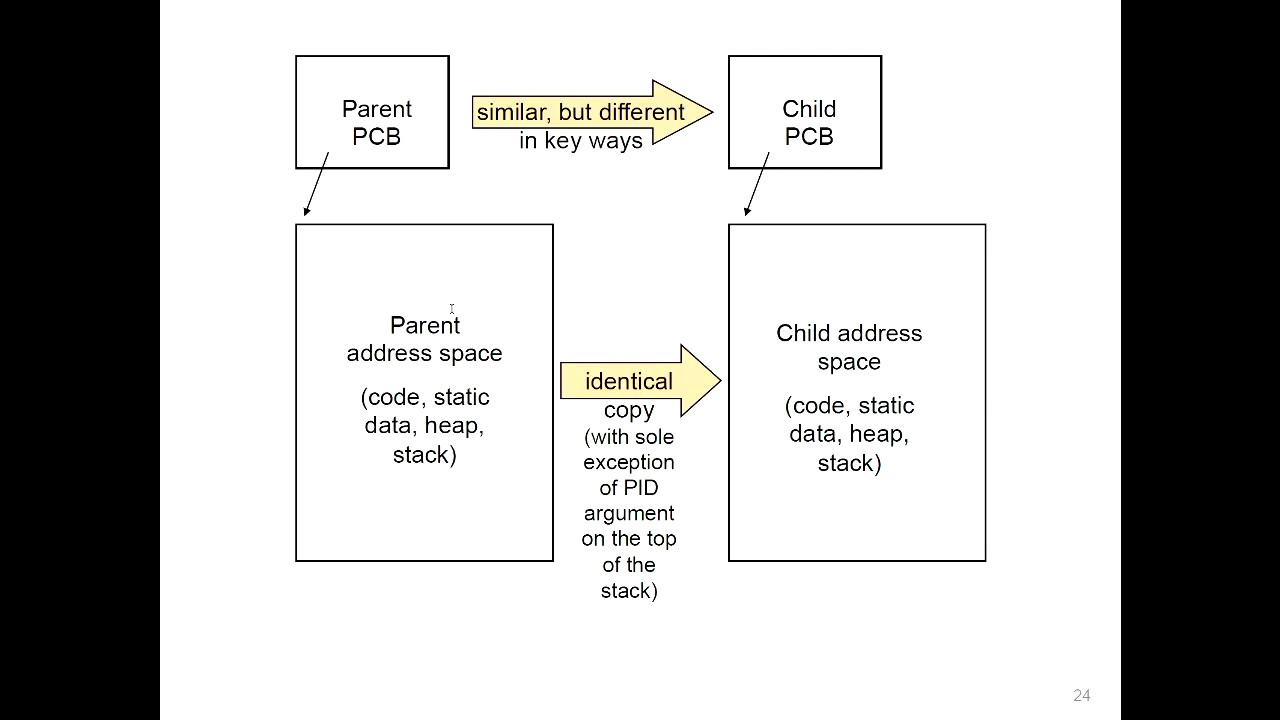
\includegraphics[height=280]{fork.jpg}

\textbf{\texttt{exec} v.s.\ \texttt{fork}}
\begin{itemize}
    \item Q:\ So how do we start a new program, instead of just forking the old program?
    \item A:\ First \texttt{fork}, then \texttt{exec}.
    \item \texttt{exec}
        \begin{itemize}
            \item stops the current process
            \item loads program `prog' into the address space
                (i.e.\ overwrites the existing process image)
            \item initialises hardware context, args for new program
            \item places PCB onto ready queue
            \item \emph{does not create a new process!}
        \end{itemize}
\end{itemize}

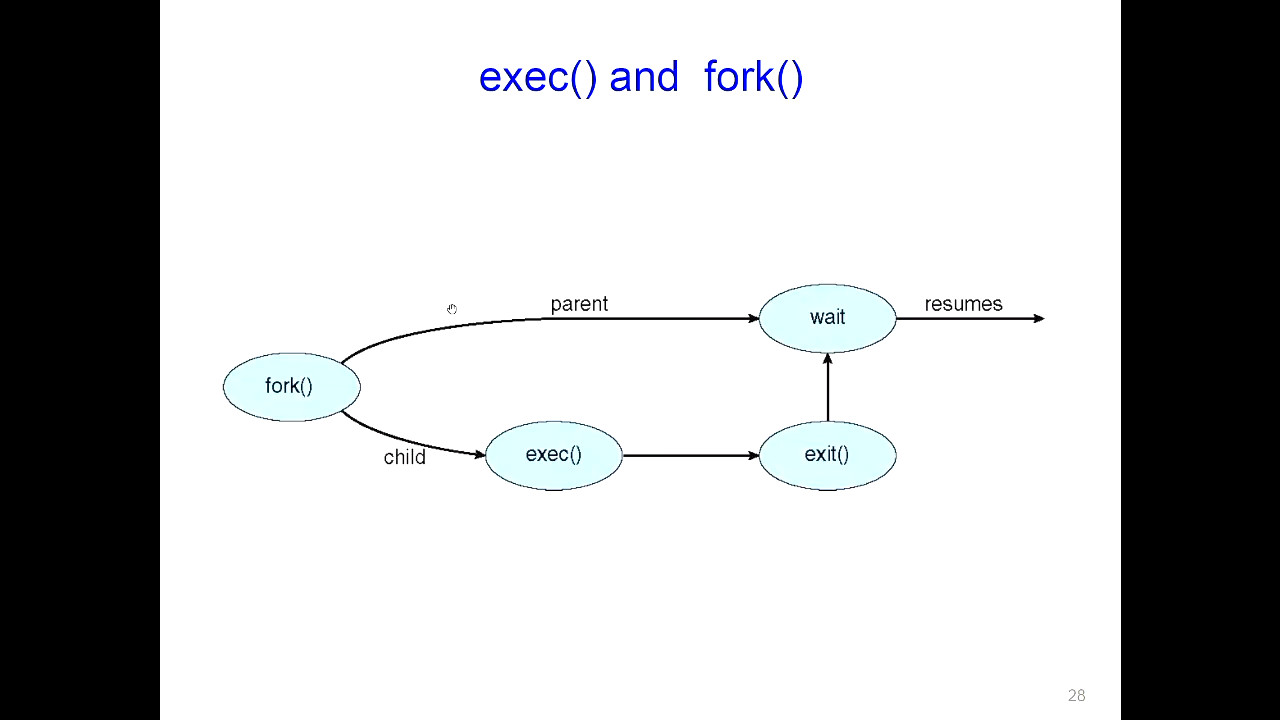
\includegraphics[height=280]{exec-and-fork.jpg}

\textbf{Method 1: \texttt{vfork}}
\begin{itemize}
    \item \texttt{vfork} is the older (now uncommon) of the two approaches.
    \item Instead of ``child's address space is a copy of the parent's'',
        the semantics are ``child's address space \emph{is} the parent's'',
        \begin{itemize}
            \item with a ``promise'' that the child won't modify the address space before doing
                an \texttt{execve}.
            \item When \texttt{execve} is called, a new address space is created and it's
                loaded with the new executable.
            \item Parent is blocked until \texttt{execve} is executed by child.
            \item Saves wasted effort of duplicating parent's address space.
        \end{itemize}
\end{itemize}

\textbf{Method 2: copy-on-write}
\begin{itemize}
    \item Retains the original semantics, but copies ``only what is necessary'' rather than
        the entire address space.
    \item On \texttt{fork}:
        \begin{itemize}
            \item Create a new address space
            \item Initialise page tables with same mappings as the parent's
                (i.e.\ they both point to the same physical memory).
                \begin{itemize}
                    \item (No copying of address space contents have occurred at this point
                --- with the sole exception of the top page of the stack.)
                \end{itemize}
            \item Set both parent and child page tables to make all pages read-only
            \item If either parent or child writes to memory, an exception occurs.
            \item When exception occurs, OS copies the page, adjusts page tables, etc.
        \end{itemize}
\end{itemize}

\subsection{Summary}
\begin{itemize}
    \item Process
    \item PCB
    \item Process state
    \item Context switch
    \item Process creation and termination
\end{itemize}

\break{}

\section{Threads}

\subsection{Process vs Threads}

\textbf{What's \emph{in} a process?}
\begin{itemize}
    \item A process consists of (at least):
        \begin{itemize}
            \item An \emph{address space}, containing
                \begin{itemize}
                    \item the code (instructions) for the running program
                    \item the data for the running program
                \end{itemize}
            \item \emph{Thread state}, consisting of
                \begin{itemize}
                    \item The PC, indicating the next instruction
                    \item The SP, indicating the position on the stack
                    \item Other general purpose registers
                \end{itemize}
            \item A set of \emph{OS resources}
                \begin{itemize}
                    \item Open files, network connections, sound channels, \dots
                \end{itemize}
        \end{itemize}
    \item Decompose \dots
        \begin{itemize}
            \item address space
            \item \emph{thread of control} (stack, SP, PC, registers)
            \item OS resources
        \end{itemize}
\end{itemize}

\textbf{Motivation}
\begin{itemize}
    \item Threads are about \emph{concurrency} and \emph{parallelism}
    \item One way to get concurrency and parallelism is to use multiple processes
        \begin{itemize}
            \item The programs (code) of distinct processes are isolated from each other
        \end{itemize}
    \item Threads are another way to get concurrency and parallelism
        \begin{itemize}
            \item Threads \emph{share a process} --- same address space, same OS resources
            \item Threads have private stack, CPU state --- are schedulable
        \end{itemize}
\end{itemize}

\textbf{What's needed?}
\begin{itemize}
    \item In many cases
        \begin{itemize}
            \item Everybody wants to run the same code
            \item Everybody wants to access the same data
            \item Everybody has the same privileges
            \item Everybody uses the same resources (open files, network connections, etc.)
        \end{itemize}
    \item But you'd like to have multiple hardware execution states:
        \begin{itemize}
            \item an execution stack and SP
                \begin{itemize}
                    \item traces state of procedure calls made
                \end{itemize}
            \item the PC, indicating the next instruction
            \item a set of general-purpose processor registers and their values
        \end{itemize}
\end{itemize}

\textbf{How could we achieve this?}
\begin{itemize}
    \item Given the process abstraction as we know it:
        \begin{itemize}
            \item for several processes
            \item cause each to \emph{map} to the \emph{same} physical memory to share data
                (\texttt{shmget}),
        \end{itemize}
    \item This is really inefficient
        \begin{itemize}
            \item space: PCB, page tables, etc.
            \item time: creating OS structures, fork/copy address space, etc.
        \end{itemize}
\end{itemize}

\textbf{Can we do better?}
\begin{itemize}
    \item Key idea:
        \begin{itemize}
            \item separate the concept of a \emph{process} (address space, OS resources)
            \item \dots from that of a minimal \emph{thread of control}
                (execution state: stack, SP, PC, registers),
        \end{itemize}
    \item This execution state is usually called a \emph{thread}, or a
        \emph{lightweight process}.
\end{itemize}

\textbf{Threads and processes}
\begin{itemize}
    \item Most modern OS\emph{s} support two entities:
        \begin{itemize}
            \item the \emph{process}, which defines the address space and general process
                attributes (such as open files, etc.)
            \item the \emph{thread}, which defines a sequential execution stream within a
                process.
        \end{itemize}
    \item A thread is bound to a single process / address space
        \begin{itemize}
            \item address spaces, however, can have multiple threads executing within them
            \item sharing data between threads is cheap: all see the same address space
            \item creating threads is cheap, too!
        \end{itemize}
    \item \emph{Threads become the unit of scheduling}
        \begin{itemize}
            \item processes / address spaces are just \emph{containers} in which threads
                execute.
        \end{itemize}
\end{itemize}

\textbf{Single and Multi-threaded Processes}
\begin{itemize}
    \item Different threads in the same process have separate registers and stacks.
    \item This is cheaper than duplicating the instructions and PCB etc.,
        as required by having multiple processes.
\end{itemize}

\subsection{Concurrency}

\textbf{Communication}
\begin{itemize}
    \item Threads are concurrent executions sharing an address space (and some OS resources)
    \item Address spaces provide isolation
        \begin{itemize}
            \item If you can't name an object, you can't read or write to it
        \end{itemize}
    \item Hence, communicating between processes is expensive
        \begin{itemize}
            \item Must go through the OS to move data from one address space to another
        \end{itemize}
    \item Because threads are in the same address space, communication is simple/cheap
        \begin{itemize}
            \item Just update a shared variable!
        \end{itemize}
\end{itemize}

\textbf{The design space}

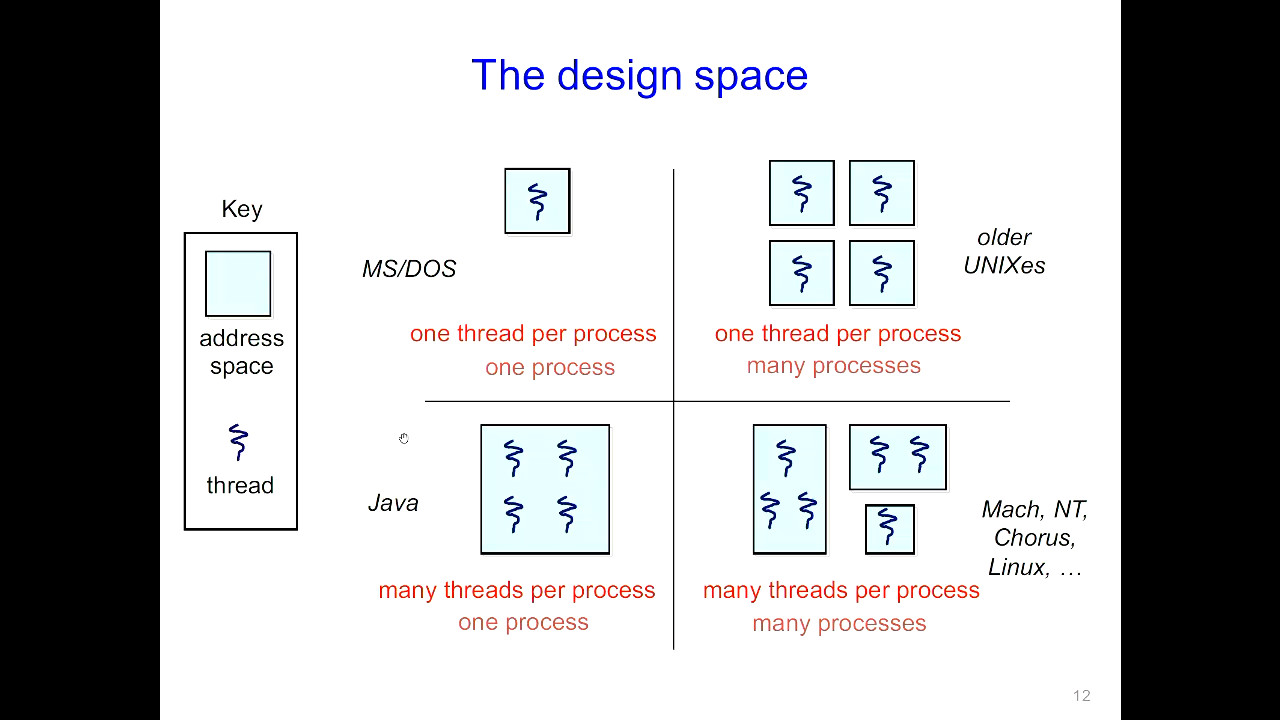
\includegraphics[height=280]{the-design-space.jpg}

\textbf{Process address space}

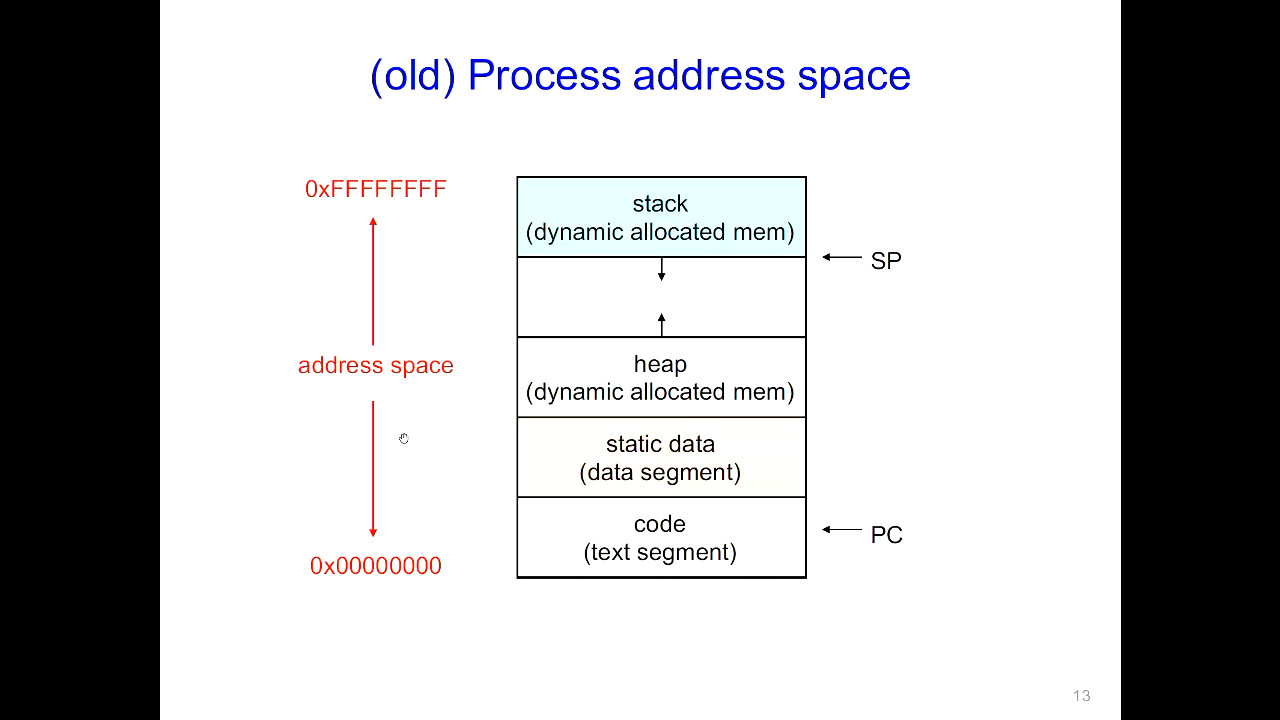
\includegraphics[height=280]{process-address-space.jpg}
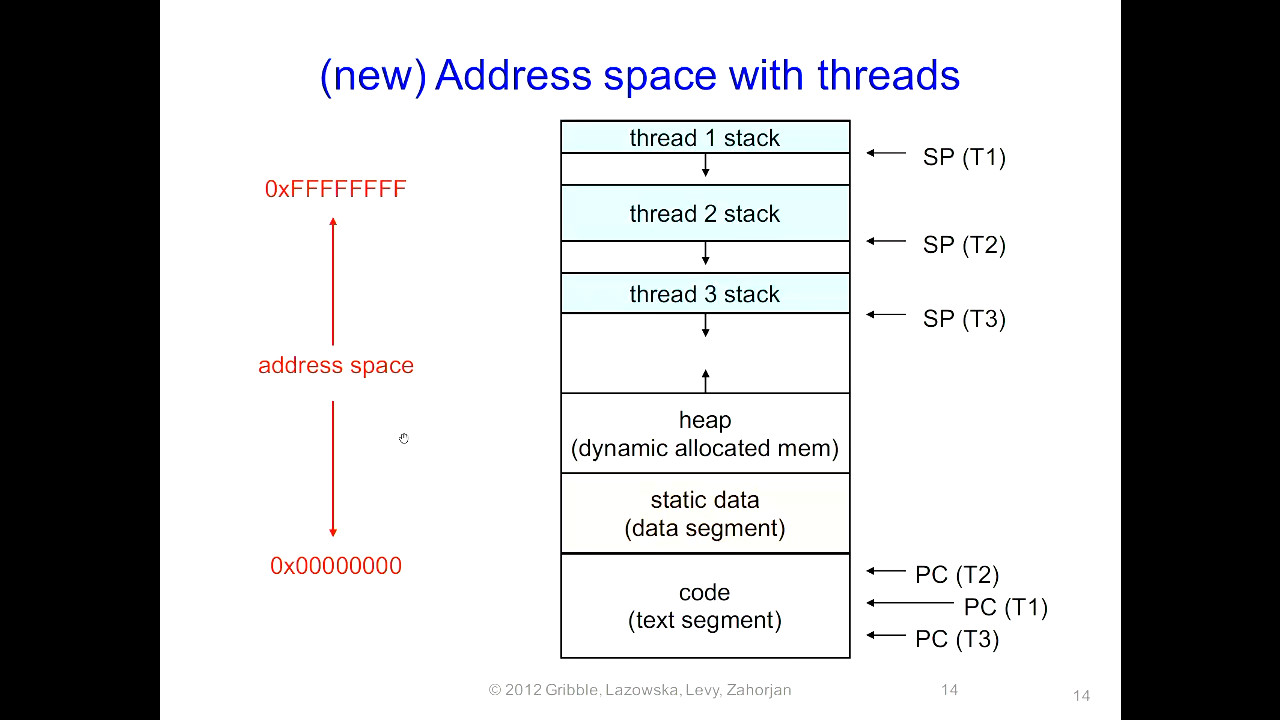
\includegraphics[height=280]{process-address-space-threads.jpg}

\subsection{Design space of process/threads}

\textbf{Process/thread separation}
\begin{itemize}
    \item Concurrency (multi-threading) is useful for:
        \begin{itemize}
            \item handling concurrent events (e.g.\ web servers and clients)
            \item building parallel programs (e.g.\ matrix multiply, ray tracing)
            \item improving program structure (the Java argument),
        \end{itemize}
    \item Multi-threading is useful even on a uniprocessor
        \begin{itemize}
            \item even though only one thread can run at a time
        \end{itemize}
    \item Supporting multi-threading --- that is, separating the concept of a \emph{process}
        (address space, files, etc.) from that of a minimal \emph{thread of control}
        (execution state), is a big win
        \begin{itemize}
            \item creating concurrency does not require creating new processes
            \item ``faster / better / cheaper''
        \end{itemize}
\end{itemize}

\subsection{Kernel threads}

\textbf{Where do threads come from?}
\begin{itemize}
    \item Natural answer: the OS is responsible for creating/managing threads \\
        For example, the kernel call to create a new thread would
        \begin{itemize}
            \item allocate an execution stack within the process address space
            \item create and initialize a \emph{Thread Control block} \\
                (SP, PC, register values)
            \item stick it on the ready queue
        \end{itemize}
    \item We call these \emph{kernel threads} \\
        There is a ``thread name space''
        \begin{itemize}
            \item Thread IDs (TIDs)
            \item TIDs are integers
        \end{itemize}
\end{itemize}

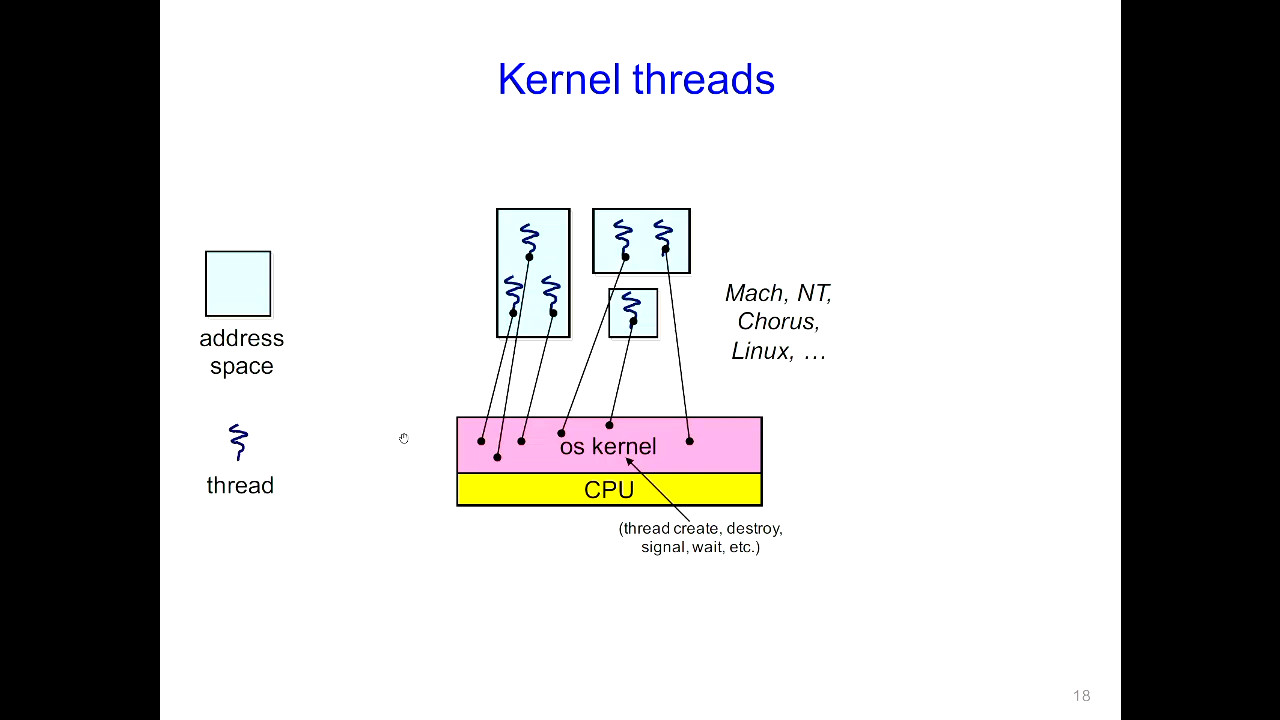
\includegraphics[height=280]{kernel-threads.jpg}

\textbf{Kernel Threads}
\begin{itemize}
    \item OS now manages threads \emph{and} processes / address spaces
        \begin{itemize}
            \item all thread operations are implemented in the kernel
            \item OS schedules all of the threads in a system
                \begin{itemize}
                    \item if one thread in a process blocks (e.g.\ on I/O),
                        the OS knows about it, and can run other threads from that process
                    \item possible to overlap I/O and computation \emph{inside} a process
                \end{itemize}
        \end{itemize}
    \item Kernel threads are cheaper than processes
        \begin{itemize}
            \item less state to allocate and initialise
        \end{itemize}
    \item But, they're still pretty expensive for fine-grained use
        \begin{itemize}
            \item orders of magnitude more expensive than a procedure call
            \item thread operations are all \emph{system calls}
                \begin{itemize}
                    \item context switch
                    \item argument checks
                \end{itemize}
            \item must maintain kernel state for each thread
        \end{itemize}
\end{itemize}

\subsection{User-level threads}

\textbf{Cheaper alternative}
\begin{itemize}
    \item There is an alternative to kernel threads
    \item Threads can also be managed at the user level (within the process)
        \begin{itemize}
            \item a library linked into the program manages the threads
                \begin{itemize}
                    \item the thread manager doesn't need to manipulate address spaces
                        (which only the kernel can do)
                    \item threads differ (roughly) only in hardware contexts
                        (PC, SP, registers), which can be manipulated by user-level code
                    \item the \emph{thread package} multiplexes user-level threads on top
                        of kernel threads
                    \item each kernel thread is treated as a \emph{virtual processor}
                \end{itemize}
            \item we call these \emph{user-level threads}
        \end{itemize}
\end{itemize}

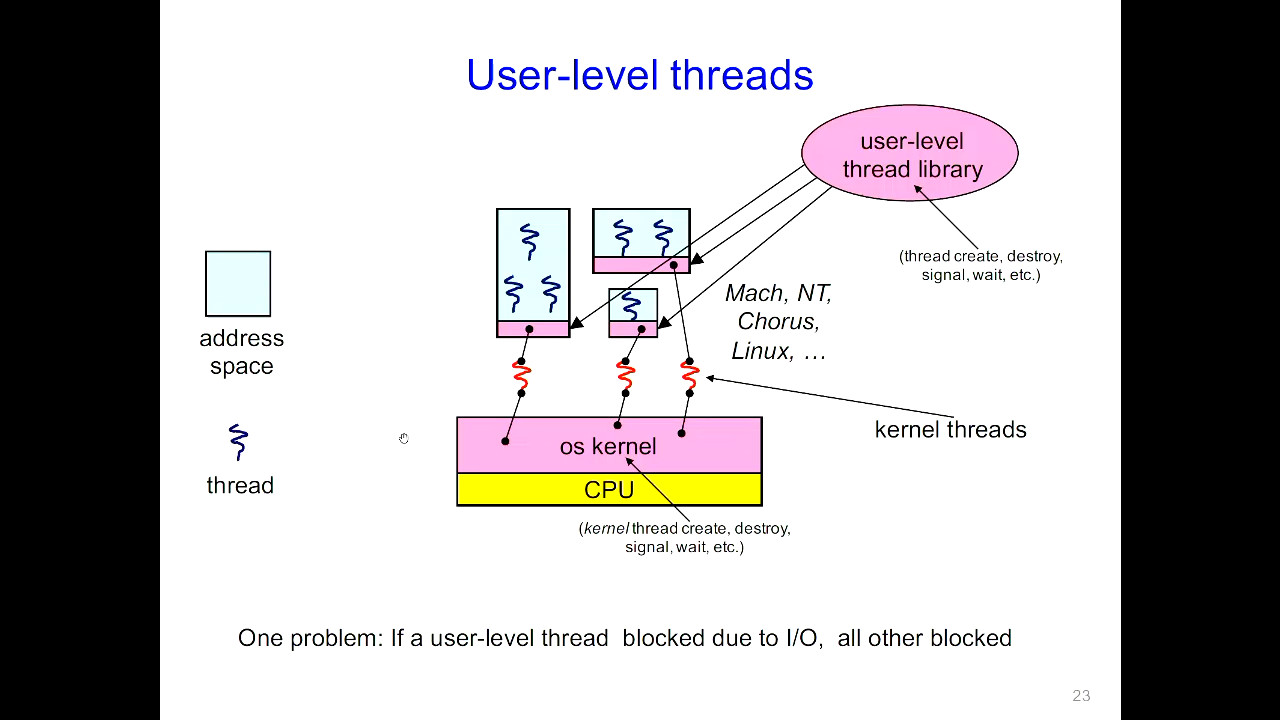
\includegraphics[height=280]{user-level-threads.jpg}

\textbf{User-level threads}
\begin{itemize}
    \item User-level threads are small and fast
        \begin{itemize}
            \item managed entirely by user-level library (e.g.\ \texttt{pthreads})
            \item each thread is represented by a PC, registers, a stack, and a small
                \emph{thread control block} (TCB)
            \item creating a thread, switching between threads, and synchronising
                threads are done \emph{via procedure calls}
                \begin{itemize}
                    \item no kernel involvement necessary!
                \end{itemize}
        \end{itemize}
    \item User-level thread operations can be 10--100x faster than kernel threads as a result.
\end{itemize}

\textbf{User-level thread implementation}
\begin{itemize}
    \item The OS schedules the kernel thread
    \item The kernel thread executes user code, including the thread support library
        and its associated thread scheduler
    \item The thread scheduler determines when a user-level thread runs
        \begin{itemize}
            \item it uses queues to keep track of what threads are doing: run, ready, wait
                \begin{itemize}
                    \item just like the OS and processes
                    \item but, implemented at user-level as a library
                \end{itemize}
        \end{itemize}
\end{itemize}

\textbf{Thread context switch}
\begin{itemize}
    \item Very simple for user-level threads:
        \begin{itemize}
            \item save context of currently running thread
                \begin{itemize}
                    \item push CPU state onto thread stack
                \end{itemize}
            \item restore context of the next thread
                \begin{itemize}
                    \item pop CPU state from next thread's stack
                \end{itemize}
            \item return as the new thread
                \begin{itemize}
                    \item execution resume at PC of next thread
                \end{itemize}
            \item Note: no changes to memory mapping required
        \end{itemize}
    \item This is all done in assembly language
        \begin{itemize}
            \item it works at the level of the procedure calling convention
        \end{itemize}
\end{itemize}

\textbf{How to keep a user-level thread from hogging the CPU?}
\begin{itemize}
    \item Strategy 1: force everyone to cooperate
        \begin{itemize}
            \item a thread willingly gives up the CPU by calling \texttt{yield}
            \item \texttt{yield} calls into the scheduler, which context switches to
                another ready thread
            \item what happens if a thread never calls \texttt{yield}?
        \end{itemize}
    \item Strategy 2: use presumption
        \begin{itemize}
            \item scheduler requests that a timer interrupt be delivered by the OS
                periodically
                \begin{itemize}
                    \item usually delivered as a UNIX signal (\texttt{man signal})
                    \item signals are just like software interrupts, but delivered to
                        user-level by the OS instead of delivered to the OS by hardware
                \end{itemize}
            \item at each timer interrupt, scheduler gains control and context switches
                as appropriate.
        \end{itemize}
\end{itemize}

\textbf{What if a thread tries to do I/O}
\begin{itemize}
    \item The kernel thread ``powering'' it is lost for the duration of (synchronous)
        I/O operation!
        \begin{itemize}
            \item The kernel thread blocks in the OS, as always
            \item It maroons with it the state of the user-level thread
        \end{itemize}
    \item Could have one kernel thread ``powering'' each user-level thread
        \begin{itemize}
            \item ``common case'' operations (e.g.\ synchronisation) would be quick
        \end{itemize}
    \item Could have a limited-size ``pool'' of kernel threads ``powering'' all the
        user-level threads in the address space
        \begin{itemize}
            \item the kernel will be scheduling these threads, obliviously to what's going
                on at user-level.
        \end{itemize}
\end{itemize}

\subsection{Summary}
\begin{itemize}
    \item Multiple threads per address space
    \item Kernel threads are much more efficient than processes, but still expensive
        \begin{itemize}
            \item all operations require a kernel call and parameter validation
        \end{itemize}
    \item User-level threads are:
        \begin{itemize}
            \item much cheaper and faster
            \item great for common-case operations
                \begin{itemize}
                    \item creation, synchronisation, destruction
                \end{itemize}
            \item can suffer in uncommon cases due to kernel obliviousness
                \begin{itemize}
                    \item I/O
                    \item pre-emption of a lock-holder
                \end{itemize}
        \end{itemize}
\end{itemize}

\section{Synchronisation}

\textbf{Temporal relations}
\begin{itemize}
    \item User view of parallel threads
        \begin{itemize}
            \item Instructions executed by a single thread are totally ordered
                \begin{itemize}
                    \item $A < B < C < \dots$
                \end{itemize}
            \item In absence of \emph{synchronisation}:
                \begin{itemize}
                    \item instructions executed by distinct threads must be considered
                        unordered / simultaneous
                    \item Not $X < X'$, and not $X' < X$
                \end{itemize}
        \end{itemize}
    \item Hardware largely supports this
\end{itemize}

\end{document}
